% !TeX root = ../main-english.tex
% !TeX spellcheck = en-US
% !TeX encoding = utf8
% -*- coding:utf-8 mod:LaTeX -*-

%This smart spell only works if no changes have been made to the chapter
%using the options proposed in preambel/chapterheads.tex.
\setchapterpreamble[u]{%
	\dictum[Albert Einstein]{If we knew what it was we were doing, it would not be called research, would it?}
}

\chapter{Reproducible state space modeling}
\label{k5}

Look mom, some text!

\section{Shared response modeling}
\pagebreak

\section{Simulation study}
\pagebreak

\section{The MEMENTO study}

The memento study investigated how decision-relevant information is retained in working memory using a decision making task with concurrent \gls{meg} acquisition.
It was acquired at the Otto-von-Guericke University Magdeburg in 2016 by \citet{kaiser}.

\subsection{Participants}

$N = 22$ right-handed, healthy participants with normal or corrected-to-normal vision took part in the experiment.
The mean age was 26 years, and 10 participants were male.
Handedness was assessed with the Edinburgh Handedness Inventory.
Participants gave their informed consent to participate in the study, and received a base monetary compensation in the order of 8€ per hour with a performance-dependent bonus.
Ethics approval was obtained from the University Clinic Magdeburg.

\subsection{Experimental design}

The experiment consisted of 510 trials, grouped into 5 blocks with a variable break in between.
Each trial required a decision between one of two stimulus options, presented as gabor patches on the left and right side of the screen (\cref{fig:memento_trial}).
Importantly, stimulus options were presented in succession, with a delay period through which the decision-relevant properties of the first stimulus had to be retained in working memory.
The number of stripes in the gabor patch encoded the reward magnitude (either 0.5, 1, 2, or 4 points), and the angle of stripes encoded reward probability (either 10\%, 20\%, 40\%, or 80\%): The more stripes, the higher the reward, and the larger the angle, the higher the probability.
Participants learned these associations in a tutorial prior to the experiment.
Each trial started with a fixation cross (1000-1900ms, jittered), followed by the first stimulus on the left side of the screen for 700ms, a 2000ms delay period through which the phrase ``or'' was presented in the center of the screen, the second stimulus option on the right side of the screen for 700ms, and a feedback screen.
Once the second stimulus option was displayed, participants chose the left or right option via a button press with the right or left index finger, respectively.
The feedback screen showed both options side by side with a frame around the chosen option, and revealed which option had been rewarded via color coding (red: unrewarded, green: rewarded).
If a decision was not made within 5 seconds, the trial was aborted and participants saw a message to respond faster.
A progress bar at the bottom of the screen tracked gains over time, resulting in a bonus payment whenever it hit a gold target line.
Participants were instructed to maximize their gains and to respond as fast as possible.
Stimulus presentation was controlled by Psychtoolbox (Cite) running on Matlab 2012b (The Mathworks Company, Natick, MA).
% taken verbatim from Lucas paper https://static-content.springer.com/esm/art%3A10.1038%2Fs41467-020-20875-w/MediaObjects/41467_2020_20875_MOESM1_ESM.pdf
All stimuli were presented on a grey background with a contrast optimized for the MEG recording chamber on a screen in a distance of one meter from the sitting participants.
Stimuli were displayed via a projector with a refresh rate of 75 Hz located outside the MEG recording chamber.

\subsection{MEG acquisition}



Memento study design here…
Neuromag MEG device with 306 sensors, active internal shielding, and head position indicator coils

fixation cross: shown between 1 and 1.9 seconds.
TODO: the reward schedule outfile\_final.mat is yet missing, the outfile in the project is outdated and contains 560 trials

\begin{figure}
	\centering
	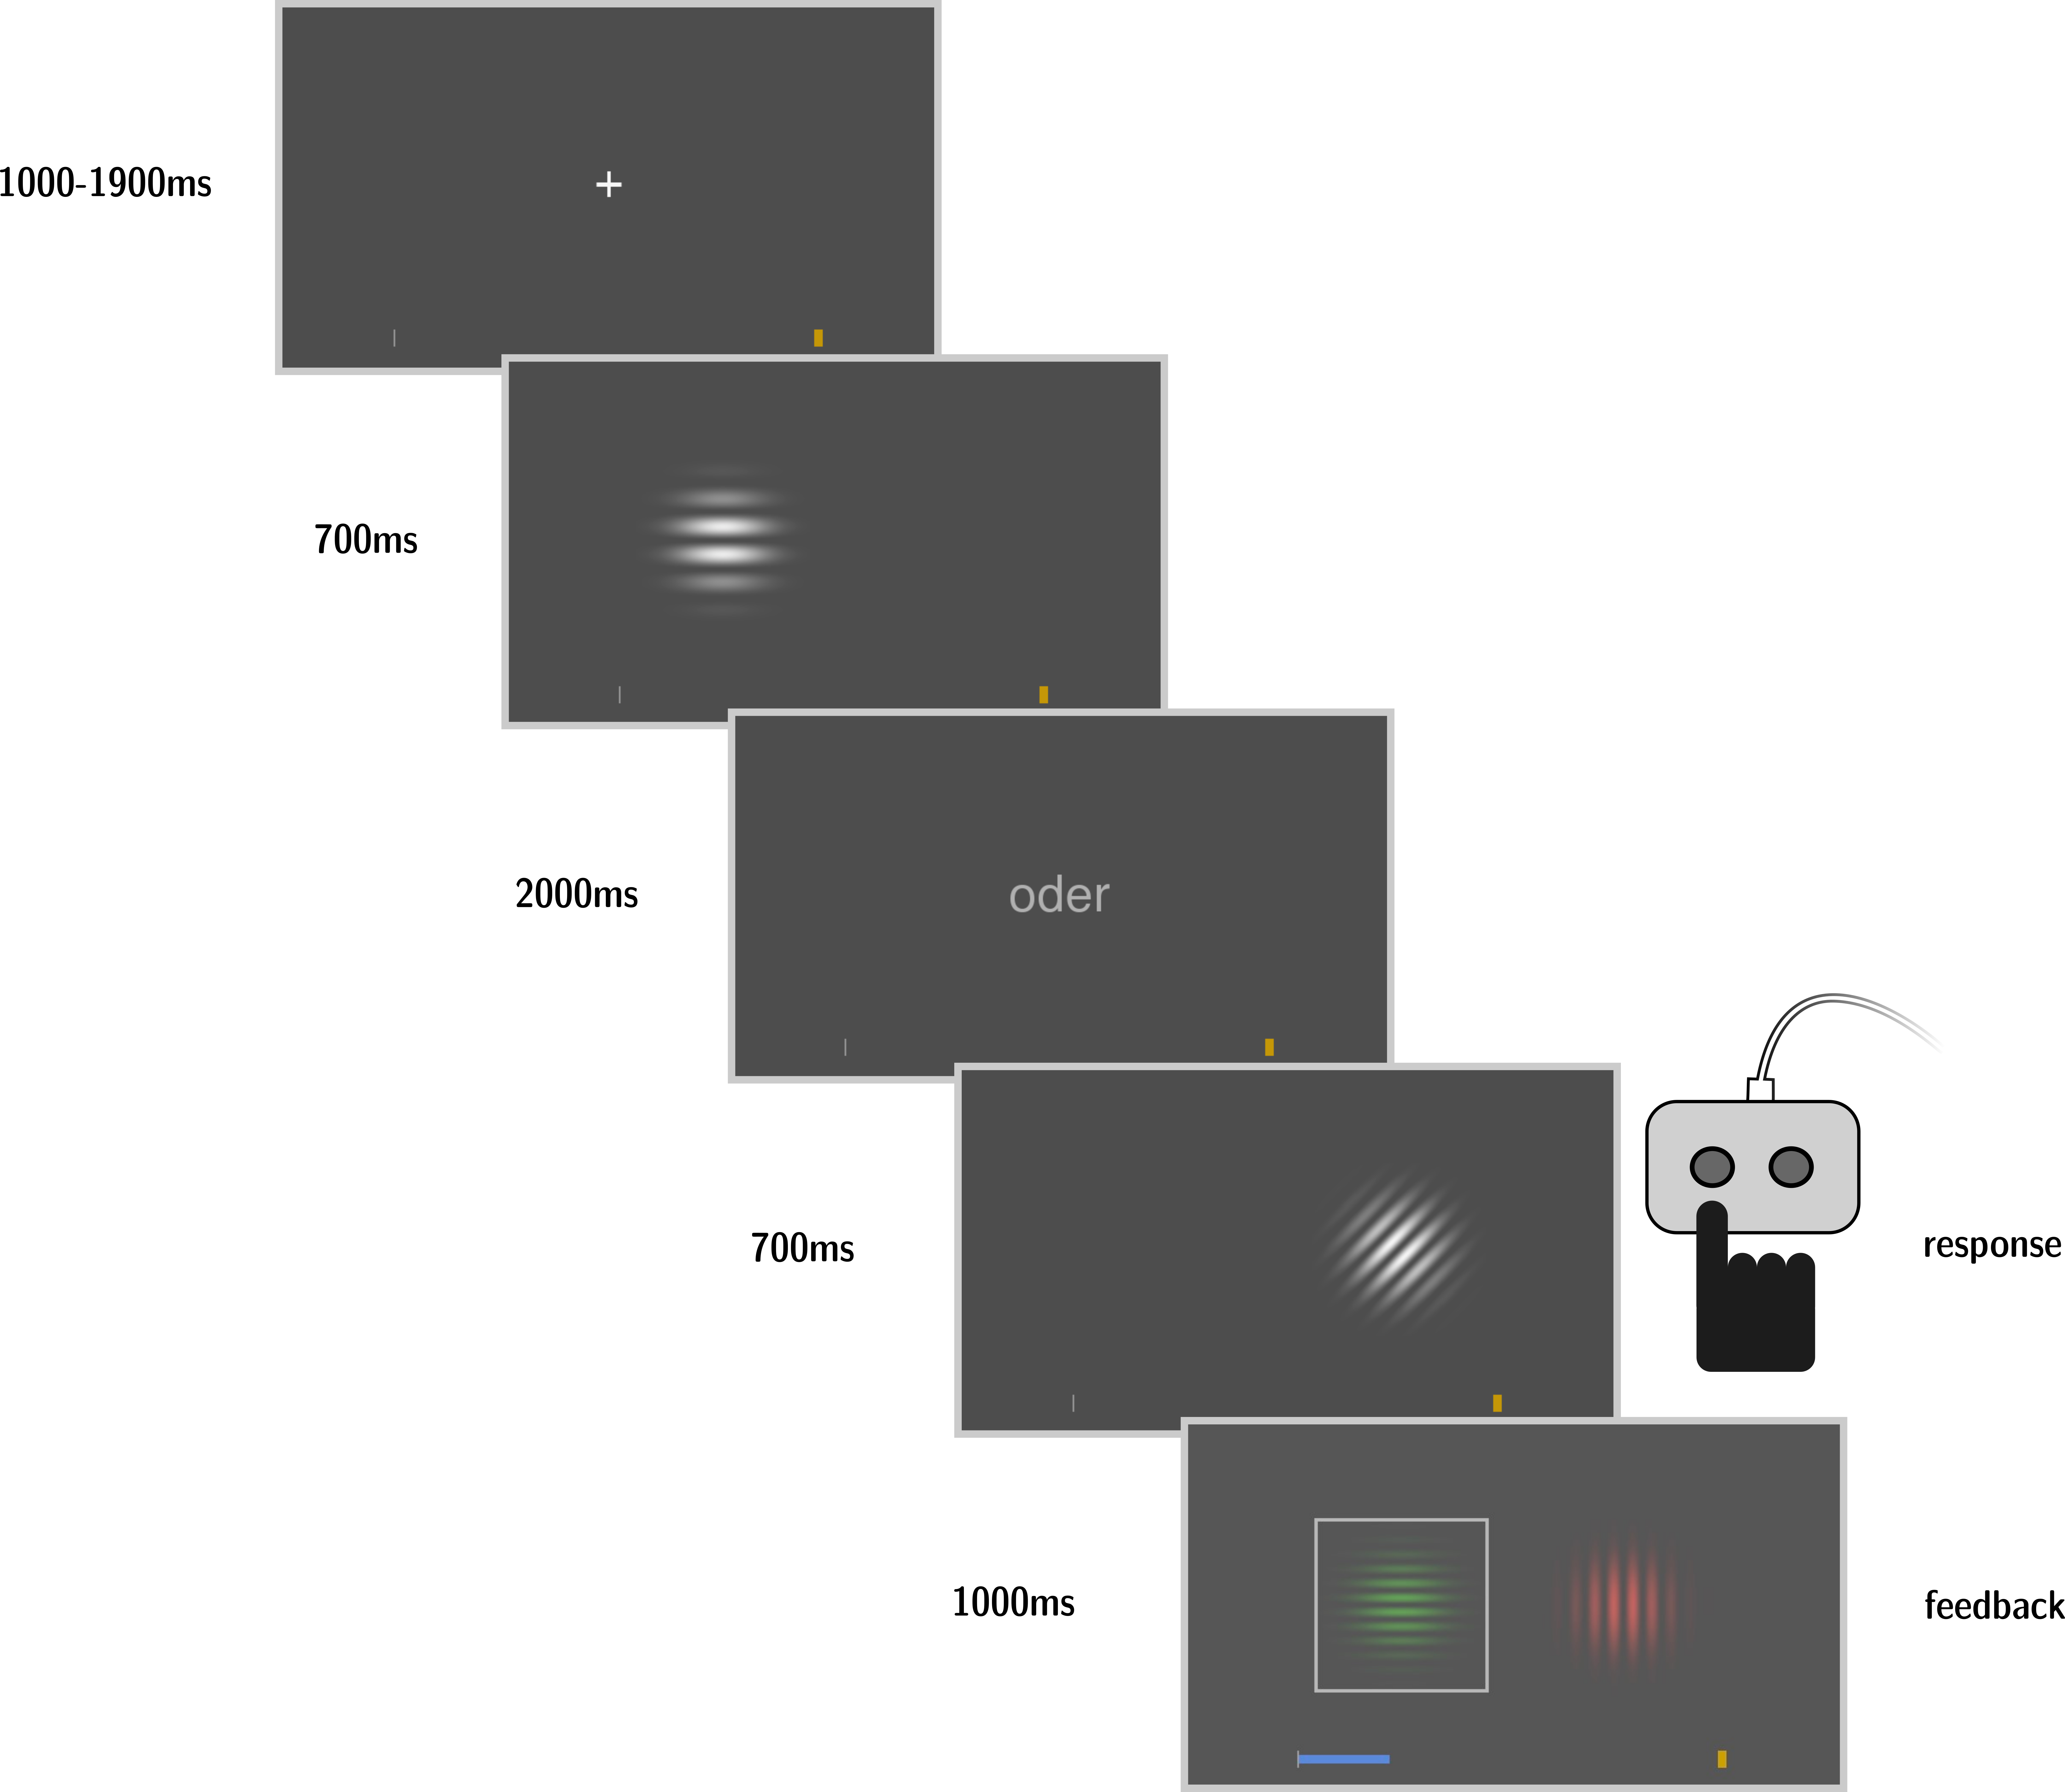
\includegraphics[width=.5\textwidth]{memento/memento_experiment.png}
	\caption[Memento: Trial overview]{Schematic overview of a single trial in the experiment.}
	\label{fig:memento_trial}
\end{figure}

\subsection{Preprocessing}

In a first step, data were restructured to BIDS format (v1.4.0) using mne-bids \citep{Appelhoff2019}.
Preprocessing consisted of the following sequential steps and is illustrated in Figure XX:
Temporal signal space separation (tsss) with movement corrections (TODO: retrieve parameters from the log files),
ZAPline filtering (CITE) to remove a ~60Hz spikes in the data, presumably from a presentation screen
Filtering (TODO: retrieve parameters from the log files)
Removal of heartbeat and eye blink artifacts with Independent component analysis (fastica)
Epoching into XXs without baseline correction. Bad epochs were interpolated or rejected using autoreject (CITE)

All preprocessing steps and the subsequent analysis were implemented using mne python (CITE) or custom Python functions. All preprocessing and analysis scripts are openly available on GitHub and as the python package \texttt{pymento\_meg} (CITE).


\pagebreak

\section{Temporal decoding}

From Grootswagers et al. (2017): MVPA for MEG/EEG
The term “multivariate pattern analysis” (or MVPA) en-
compasses a diverse set of methods for analyzing neuro-
imaging data. The common element that unites these
approaches is that they take into account the relation-
ships between multiple variables (e.g., voxels in fMRI or
channels in MEG/EEG), instead of treating them as inde-
pendent and measuring relative activation strengths. The
term “decoding” refers to the prediction of a model from
the data (“encoding” approaches do the reverse, predict-
ing the data from the model, reviewed in Naselaris, Kay,
Nishimoto, \& Gallant, 2011; see also, e.g., Ding \& Simon,
2012, for an example of encoding models for MEG). The
most common application of decoding in cognitive neu-
roscience is the use of machine learning classifiers (e.g.,
correlation classifiers (Haxby et al., 2001) or discriminant
classifiers (Carlson et al., 2003; Cox \& Savoy, 2003) to
identify patterns in neuroimaging data, which correspond
to the experimental task or stimulus. The most popular
applications of MVPA are decoding (for recent reviews on
fMRI decoding, see e.g., Haynes, 2015; Pereira et al., 2009)
and, more recently, representational similarity analysis
(RSA: Kriegeskorte \& Kievit, 2013).

\subsection{machine learning concepts in scikit-learn}

\texttt{y} is the \textit{target}, also called \texttt{outputs}, \texttt{responses}, \texttt{label} or \texttt{ground truth}.¸ Its the \texttt{dependent variable} in supervised learning, passed to an \texttt{estimator}'s fit method as y.
\texttt{X} is the observed data. Its number of rows are the number of \texttt{samples}.
\texttt{features} are the individual elements of a vector representing a sample. In a data matrix, features are represented as columns. Elsewhere features are also known as attributes, predictors, regressors, or independent variables.
\texttt{samples} typically denote a single feature vector. Elsewhere, a sample is called an instance, data point, or observation. \texttt{n\_samples} indicates the number of samples in a dataset, being the number of rows in a data array \texttt{X}


A \texttt{classifier} is a predictor with a finite set of discrete possible output values, and must implement "fit", "predict", and "score" methods, and could implement "decision\_function", "predict\_proba" and "predict\_log\_proba" methods.
An \texttt{estimator} is an object that manages the estimation and decoding of a model. An estimators fit method takes samples X, target y, and sample properties (e.g., weights). Once fitted, the "predict\_proba" method can return probability estimates for each class from some input data X. A \texttt{score} is a method that evaluates predictions on a given dataset, returning a single

\texttt{evaluation metrics} accept a ground truth and a prediction (e.g., output of predict, predict\_proba, etc)

\texttt{Transformers} (or \texttt{transforms}) can clean, reduce, expand, or generate feature representation.
 is
\texttt{Pipelines} sequentially chain transforms with a final estimator, and reduce the possibilities of forgetting transformations that could lead to inconsistent preprocessing applications between training and testing data and of leaking test data into training data. The purpose of a pipeline is to assemble several steps that can be cross-validated together whiule

\section{Results}
\pagebreak

